\documentclass[a4paper,DIV=12,english]{scrartcl}
\usepackage[utf8]{inputenc}
\usepackage{fancyhdr}
\usepackage{bookmark}
\usepackage{graphicx}
\usepackage{hyperref}
\usepackage{xurl}
\usepackage[sorting=none, style=numeric-comp]{biblatex}
\addbibresource{ref.bib}
\usepackage{csquotes}
\usepackage[dvipsnames]{xcolor}
\usepackage[num]{isodate}
\usepackage{amsthm}
\usepackage{amssymb}
\usepackage{bbm}
\usepackage{amsmath}
\usepackage{tikz}
%\usepackage{pgfplots}
    %\usepgfplotslibrary{fillbetween}
\usepackage{svg}
\usepackage{braket}
\usepackage{caption}
\usepackage{subcaption}
\usepackage{placeins}
%\setlength\parindent{0pt}
\usepackage{wrapfig}
\usepackage{float}


% Fakesection
\newcommand{\fakesection}[1]{%
    \par\refstepcounter{section}                                        % Increase section counter
    \sectionmark{#1}                                                    % Add section mark (header)
    \addcontentsline{toc}{section}{\protect\numberline{\thesection}#1}  % Add section to ToC
    % Add more content here, if needed.
} 

\renewcommand{\footrulewidth}{0.5pt}
\pagestyle{fancy}
\fancyhf{}
\fancyhead[L]{\leftmark}
\fancyhead[R]{}

\fancyfoot[C]{Computational Physics: Quantum Monte Carlo}
\fancyfoot[R]{\thepage}

\title{Computational Physics: Quantum Monte Carlo}
\author{Stockholm University, Spring Term 2024 \\Max Maschke}
\date{Apr 18 2024}


\begin{document}
\maketitle


\tableofcontents
\newpage


\newpage
\section{Introduction}
The aim of this project is to implement the variational method using Monte Carlo approximation of the ground state energy for a two body system of interacting fermions. It is part of the coursework for the computational physics class held at Stockholm University in 2024.

\section{Variational Methods and Monte Carlo Approximation}
The Hilbert spaces of quantum many body systems have a particularly nasty property: They grow exponentially in dimension with the number of particles. For example, a fermionic lattice system's Hilbert space dimension scales as $N^4$ where $N$ is the number of lattice sites. This strongly limits the applicability of exact diagonalisation methods to many body problems.
Instead, one might approach the task from another angle: The variational principle guarantees that the ground state is the unique solution to minimisation of the functional $E(\psi)$,
\begin{equation}
    E(\psi) = \frac{\braket{\psi|\mathcal{H}|\psi}}{\braket{\psi|\psi}},
\end{equation}
where $\mathcal{H}$ is the Hamiltonian.

If one chooses a trial state $\psi(\alpha)$ where $\alpha$ is a (or a set of) variational parameters, the best approximation to the ground state is given for
\begin{equation}
    \alpha = \text{argmin}_\alpha\, E(\psi(\alpha)).
\end{equation}
However, care must be taken to ensure that the trial function can actually approximate the true ground state reasonably well. This is where the true difficulty of variational methods lies. Some guidance can be found by ensuring the trial function obeys the correct symmetries of the system and has the correct statistics, i.e.\ fermionic for fermions and bosonic for bosons.

There is another issue, though: How does one calculate $E(\psi)$ for a given state? In real space representation, this is an $N\cdot d$-dimensional integral where $N$ is the number of particles and $d$ is the number of spatial dimensions. The sign problem makes numerical estimation of these integrals difficult for many particles. For a few particles, one may efficiently approximate the integral using Monte Carlo approximation.

In this project, we implement a variation of the metropolis algorithm, which can be summarised like this:
\begin{enumerate}
    \item Randomly initialise $\vec{x} = (x_{1,1}, \dots, x_{d,N})$.
    \item For each coordinate $x_{i,j}$ take a random step drawn from a normal distribution with zero mean. Accept the step if it lowers the energy. If it increases the energy, accept it with probability
    \begin{equation}
        p = \frac{|\psi_\text{new}|^2}{|\psi_\text{old}|^2}.
    \end{equation}
    \item After a set number of steps, average the energies of all positions visited.
\end{enumerate}
In practice, we do not record the energy for the first $10\%$ of steps to let it settle.

We apply the method described above to two systems:
\begin{itemize}
    \item The 1d, 1 particle harmonic oscillator
    \item A 2d, 2 particle harmonic oscillator with coulomb-like repulsion parametrised by the constant $\lambda$
\end{itemize}
The trial wave functions and expressions for the local energy may be taken from the assignment sheet. The minimisation is done using golden search, essentially an improved version of bisection, for which we omit a description here.

\section{Implementation and Numerics} 
The method is implemented as a class \texttt{monte\_carlo} in \texttt{C++}, the code can be found at~\cite{github} and is also enclosed with this report.

Random numbers are generated using a \texttt{std::random\_device}-initialised \texttt{std::std::mt19937\_64} pseudo RNG. A standard deviation of the step length normal distribution of 0.1 was observed to give good results for $4\cdot10^7$ steps.

Unfortunately, there was not enough time to study the dependence of the minimisation results on the number of steps. We use 30 golden search steps for the minimisation unless specified otherwise.

\FloatBarrier
\section{Results}
\subsection{One-particle problem}
We keep this section intentionally brief because we spent an extensive amount of time on the one-dimensional harmonic oscillator in last week's project.
\begin{figure}
    \centering
    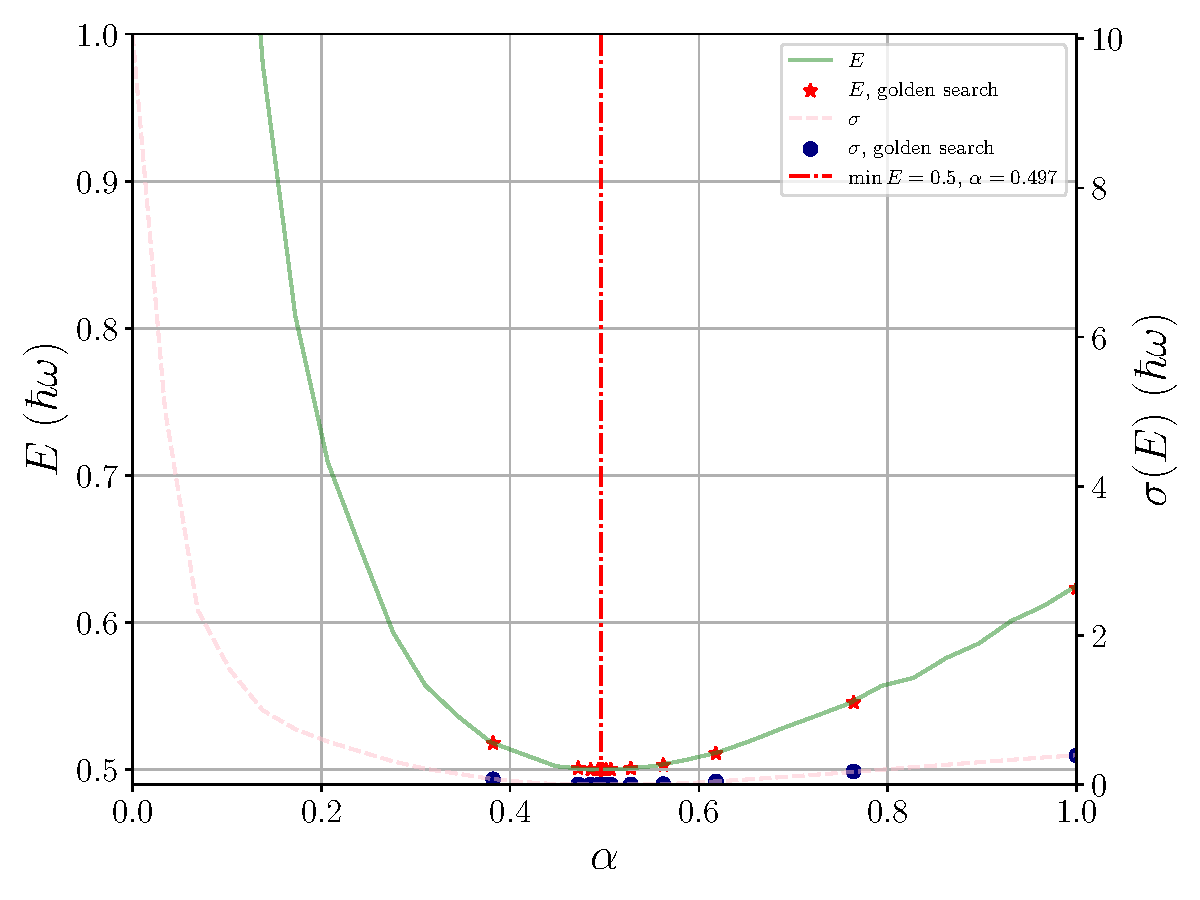
\includegraphics[width=0.65\textwidth]{../plots/summary/summary_1d.pdf}
    \caption{Minimisation of the Monte Carlo energy for the 2 particle system using golden search. The exact result $\alpha=0.5$ is replicated up to the second digit.}
    \label{fig:summary1sd}
\end{figure}
The result of the energy minimisation is shown in figure~\ref{fig:summary1sd} and reproduces the expected result of $\alpha=0.5$, $E_\text{min}=0.5\hbar\omega$ to two digits in $\alpha$ and to high precision in $E$.

We omit a plot of the wave function.

\FloatBarrier
\subsection{Two-particle problem}
The result of the minimisation for different $\lambda$ are summarised in table~\ref{tab:results} and plotted in figure~\ref{fig:summary_2d}. For $\lambda=0$ and $\lambda=1\hbar\omega$, we obtain the exact results to good accuracy.

We observe that for $\lambda=0$, since the trial function does not depend on $\alpha$, there is no true minimum since $E(\alpha)$ is constant. Increasing $\lambda$ increases the energy scale of the system. The minimising variational parameter increases with increasing $\lambda$ as well since $\alpha$ encodes the separation of the particles, intuitively speaking, and we expect stronger repulsion for higher $\lambda$. This can also be seen in figure~\ref{fig:sweep}.

Interestingly, for low $\lambda$, the standard deviation of the energy is numerically zero for $\alpha_\text{min}$ while this is no longer the case from $\lambda=2\hbar\omega$.

\begin{table}
    \centering
    \caption{Numerically obtained minimum energies and minimising variational parameters for different repulsion constants.}
    \vspace{0.25cm}
    \begin{tabular}{c|c|c}
        $\lambda$ & $E_\text{min}$ $(\hbar\omega)$ & $\alpha_\text{min}$\\
        \hline
        0 & 2.000 & n.A. \\
        1 & 3.000 & 0.382\\
        2 & 3.723 & 0.462 \\
        8 & 6.644 & 0.641 \\
    \end{tabular}
    \label{tab:results}
\end{table}
\begin{figure}
    \centering
    \begin{subfigure}{0.49\textwidth}
        \centering
        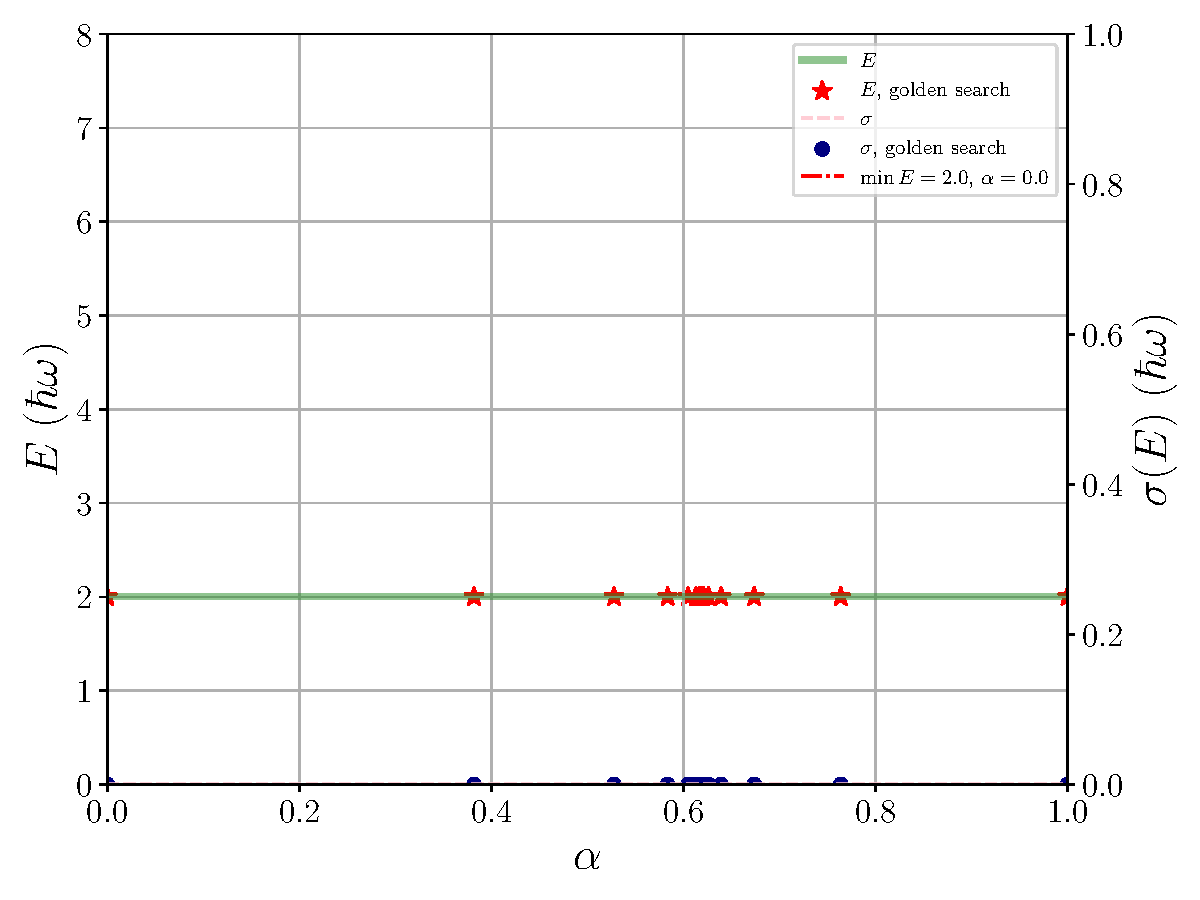
\includegraphics[width=\textwidth]{../plots/summary/summary_2d_lambda0.pdf}
        \caption{$\lambda=0\hbar\omega$}
        \label{subfig:summary_lambda0}
    \end{subfigure}
    \begin{subfigure}{0.49\textwidth}
        \centering
        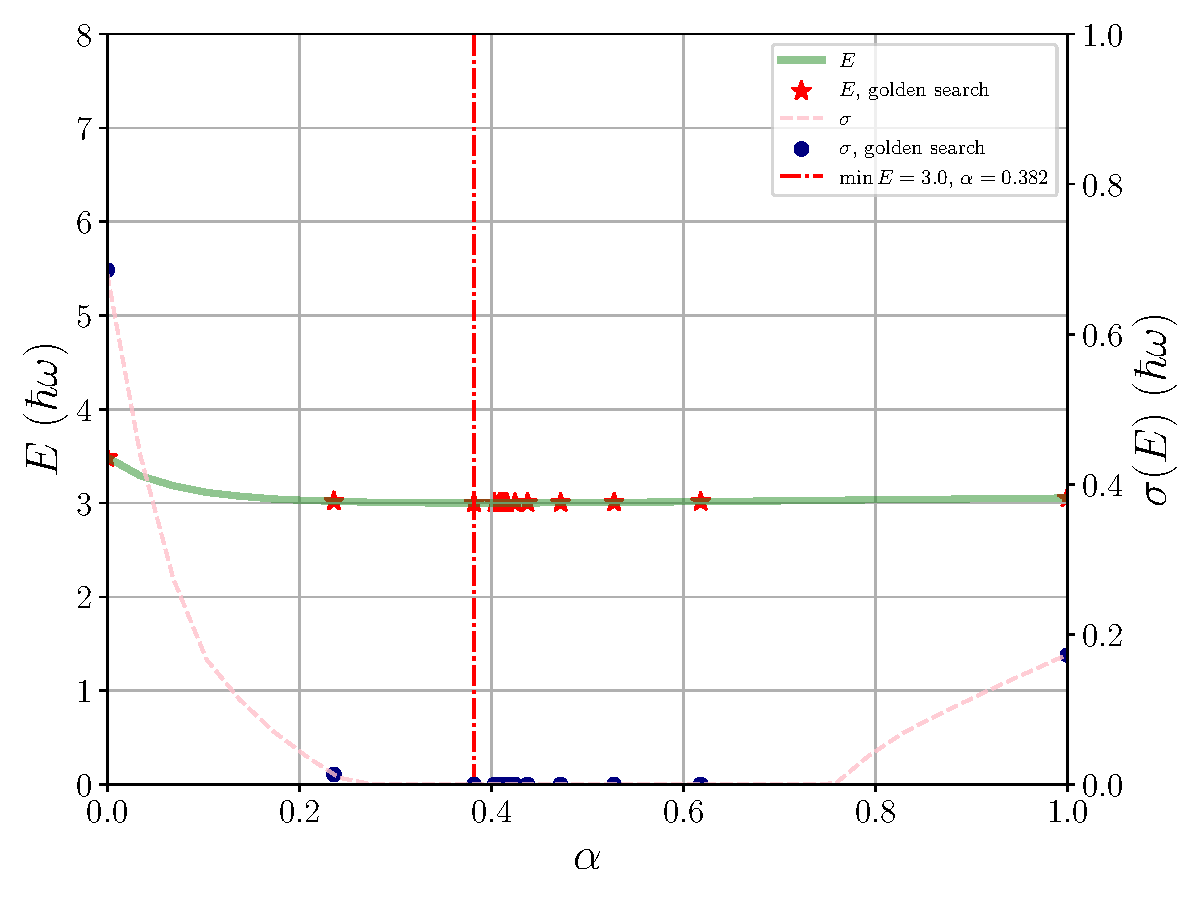
\includegraphics[width=\textwidth]{../plots/summary/summary_2d_lambda1.pdf}
        \caption{$\lambda=1\hbar\omega$}
        \label{subfig:summary_lambda1}
    \end{subfigure}\\
    \begin{subfigure}{0.49\textwidth}
        \centering
        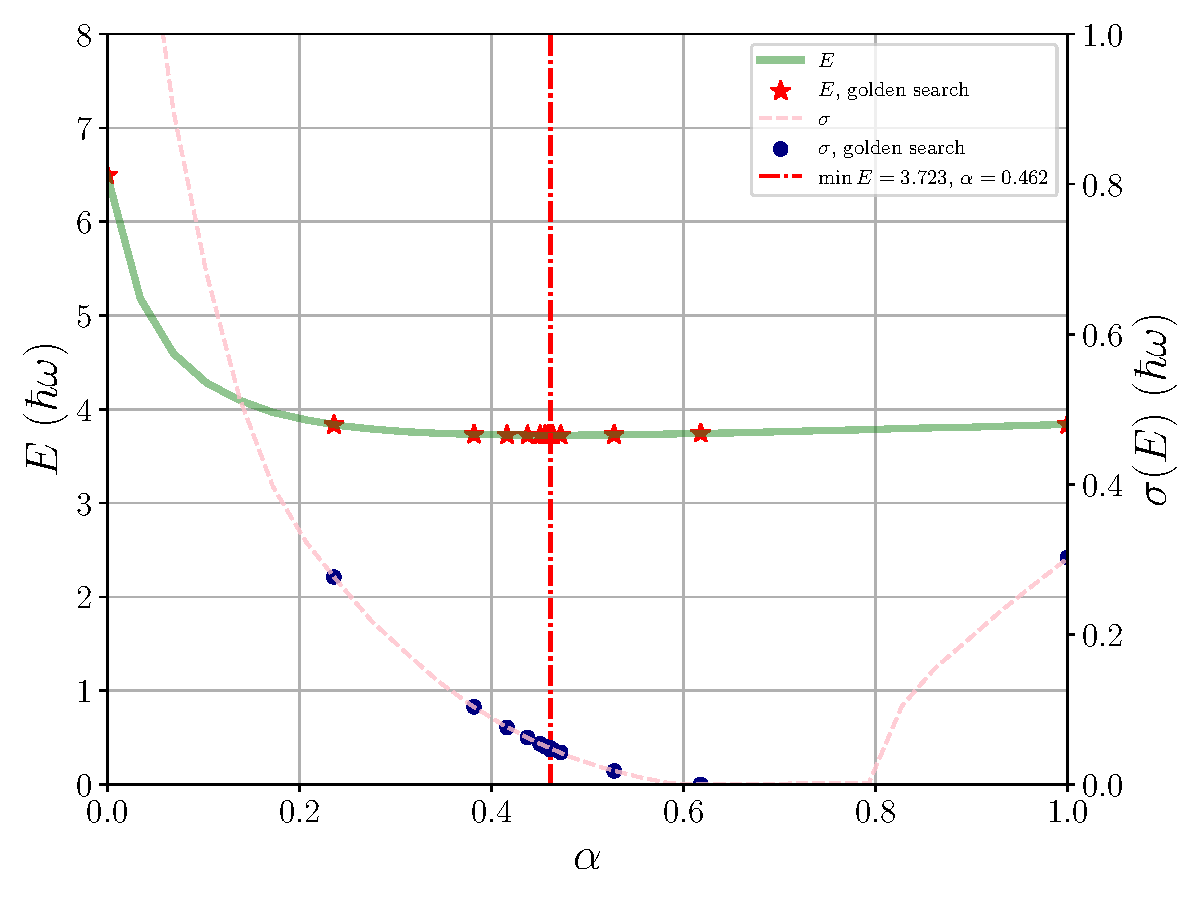
\includegraphics[width=\textwidth]{../plots/summary/summary_2d_lambda2.pdf}
        \caption{$\lambda=2\hbar\omega$}
        \label{subfig:summary_lambda2}
    \end{subfigure}
    \begin{subfigure}{0.49\textwidth}
        \centering
        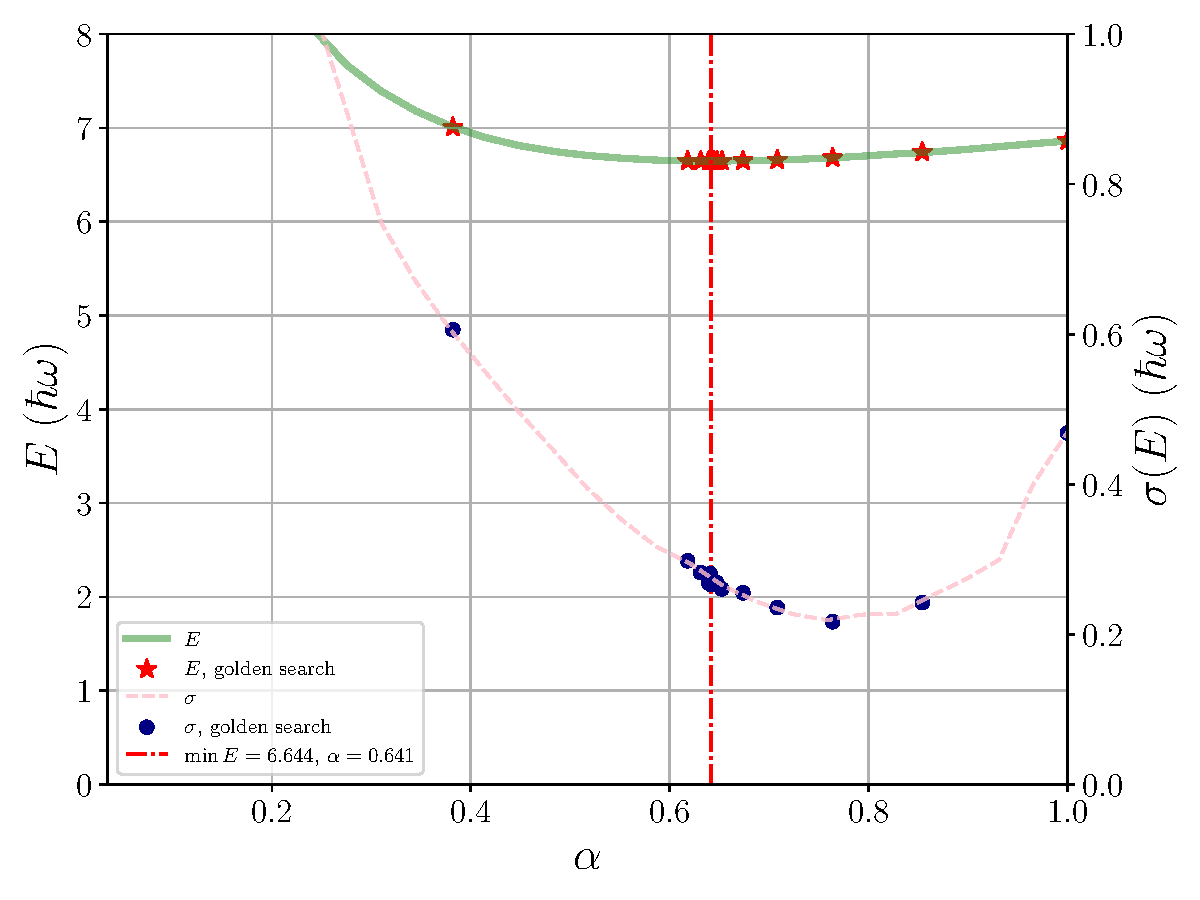
\includegraphics[width=\textwidth]{../plots/summary/summary_2d_lambda8.pdf}
        \caption{$\lambda=8\hbar\omega$}
        \label{subfig:summary_lambda8}
    \end{subfigure}
    \caption{Minimisation of the Monte Carlo energy for the 2 particle system using golden search for different repulsion constants $\lambda$. For $\lambda=0$, the trial function does not depend on $\alpha$ which thus also applies to the energies, cf.~\ref{subfig:summary_lambda0}. The minimum energy appears to scale with $\lambda$ in some way, which is to be expected.}
    \label{fig:summary_2d}
\end{figure}
\begin{figure}
    \centering
    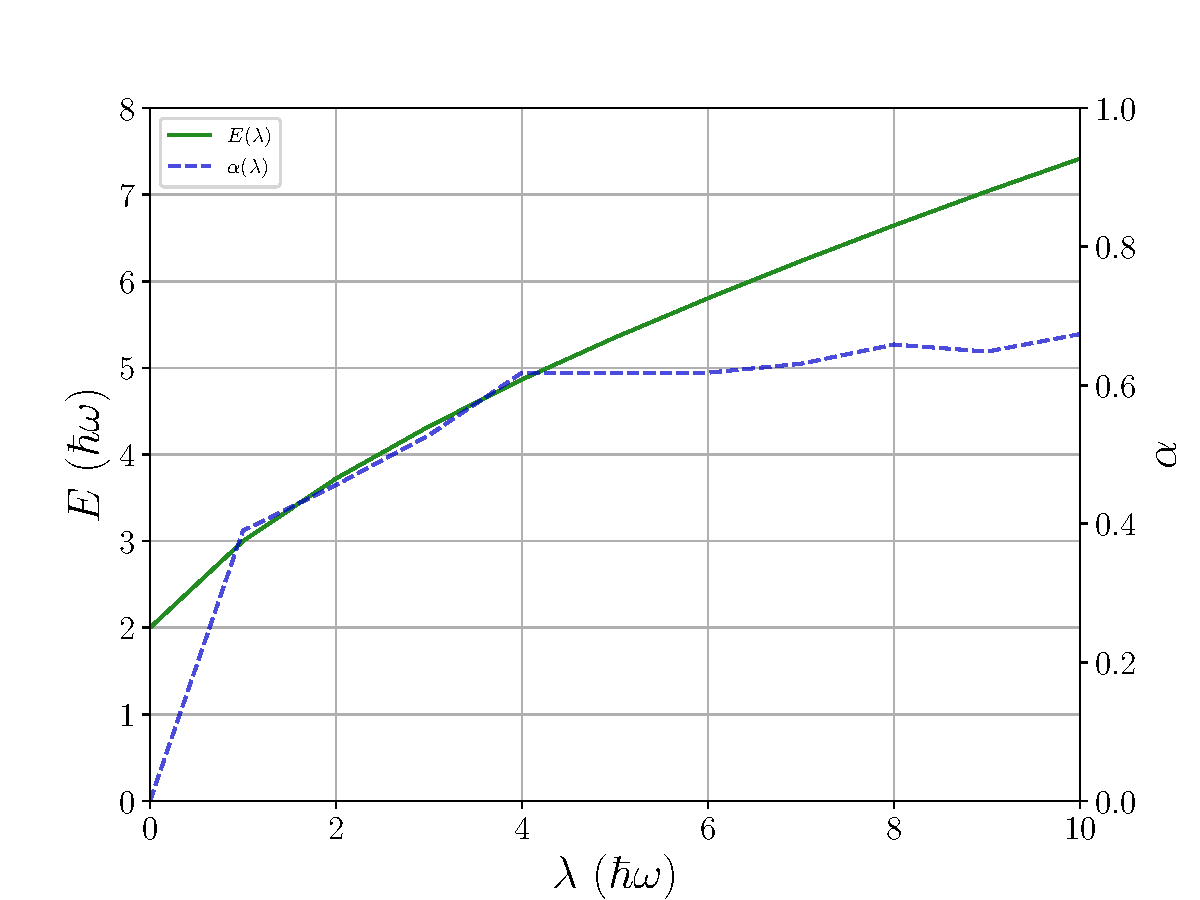
\includegraphics[width=0.65\textwidth]{../plots/sweep.pdf}
    \caption{Variation of the minimum energy $E$ and minimising $\alpha$ for different repulsion strengths $\lambda$. For this plot, only 20 golden search steps were used to reduce execution time.}
    \label{fig:sweep}
\end{figure}
\begin{figure}
    \centering
    \begin{subfigure}{0.32\textwidth}
        \centering
        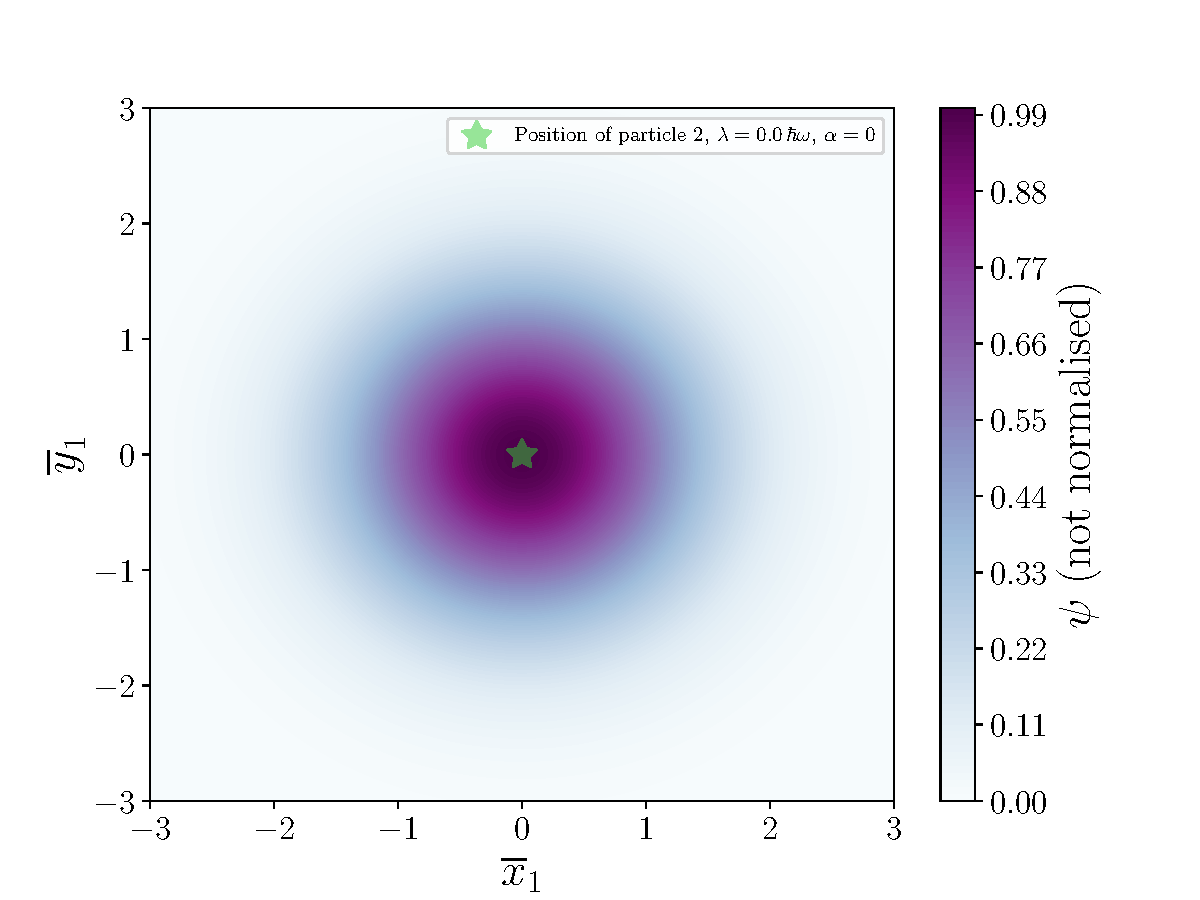
\includegraphics[width=\textwidth]{../plots/wf/wf_0_0_lambda0.pdf}
        \caption{$\lambda=0, \vec{x}_2 = (0, 0)$}
        \label{subfig:wf_0_0_0}
    \end{subfigure}
    \begin{subfigure}{0.32\textwidth}
        \centering
        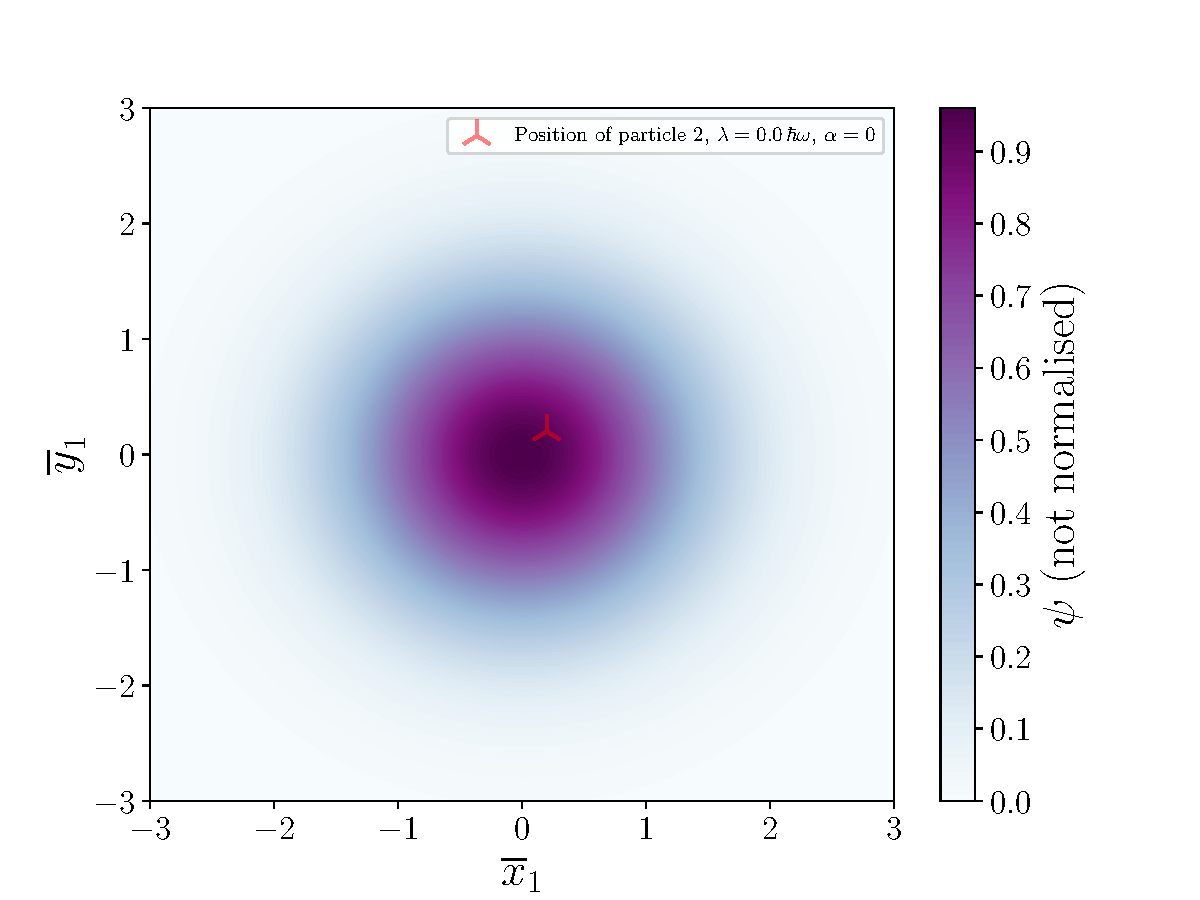
\includegraphics[width=\textwidth]{../plots/wf/wf_02_02_lambda0.pdf}
        \caption{$\lambda=0, \vec{x}_2 = (0.2, 0.2)$}
        \label{subfig:wf_02_02_0}
    \end{subfigure}
    \begin{subfigure}{0.32\textwidth}
        \centering
        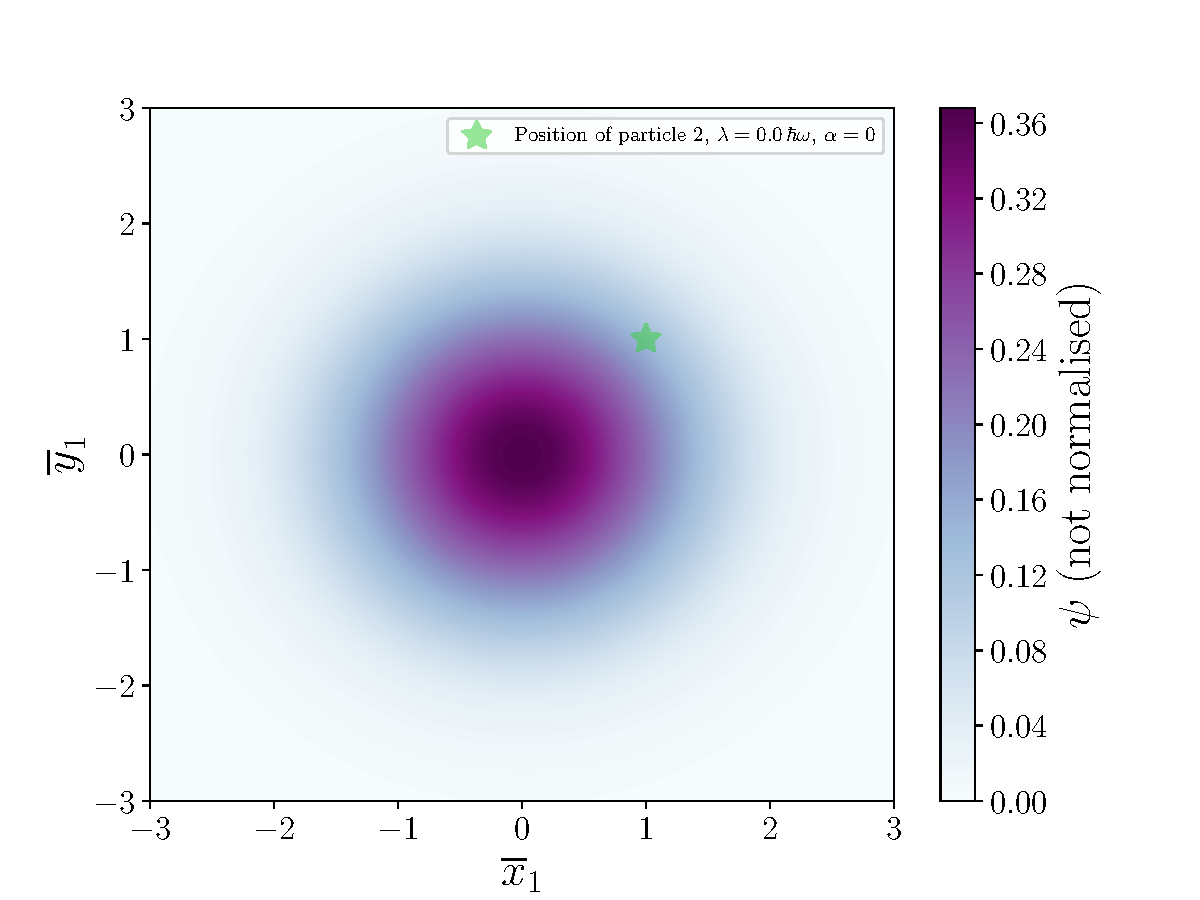
\includegraphics[width=\textwidth]{../plots/wf/wf_1_1_lambda0.pdf}
        \caption{$\lambda=0, \vec{x}_2 = (1, 1)$}
        \label{subfig:wf_1_1_0}
    \end{subfigure} \\
    \begin{subfigure}{0.32\textwidth}
        \centering
        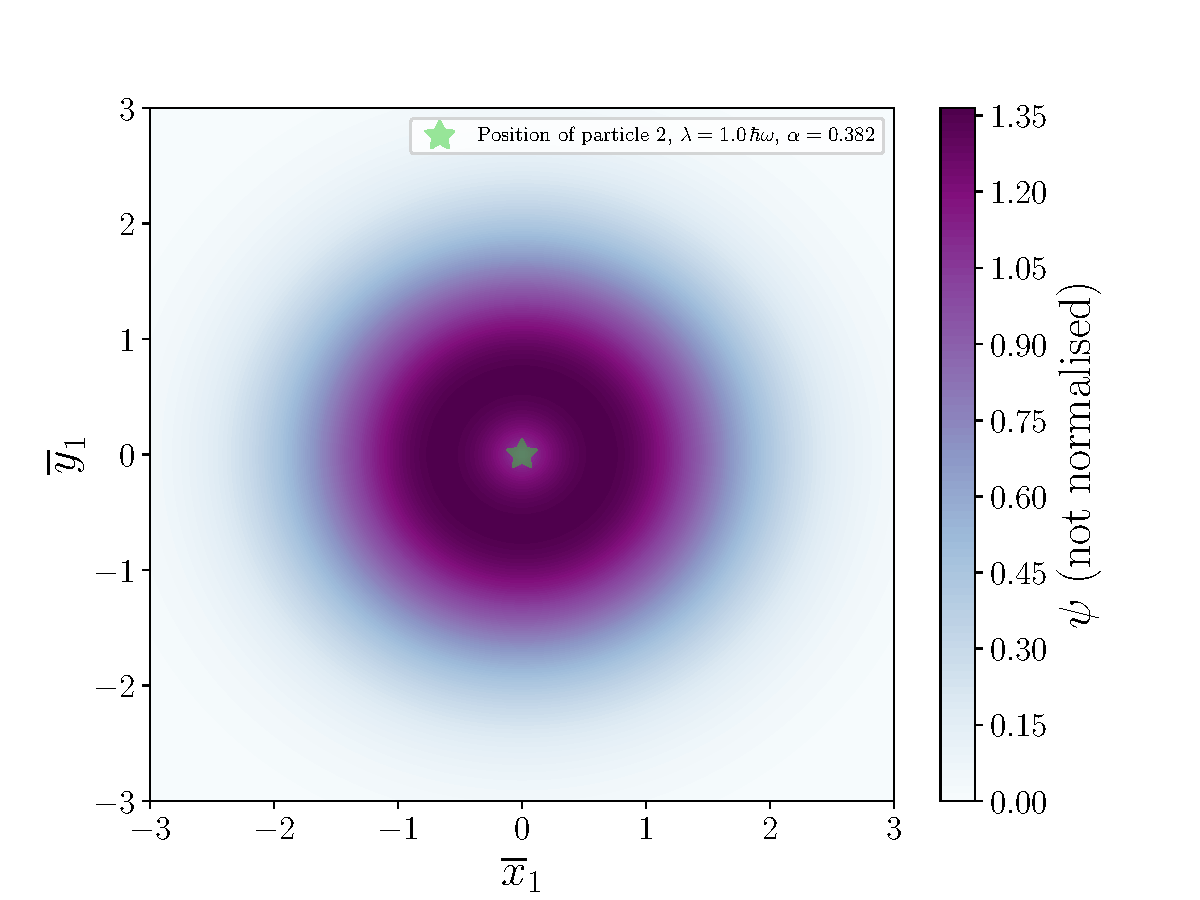
\includegraphics[width=\textwidth]{../plots/wf/wf_0_0_lambda1.pdf}
        \caption{$\lambda=1, \vec{x}_2 = (0, 0)$}
        \label{subfig:wf_0_0_1}
    \end{subfigure}
    \begin{subfigure}{0.32\textwidth}
        \centering
        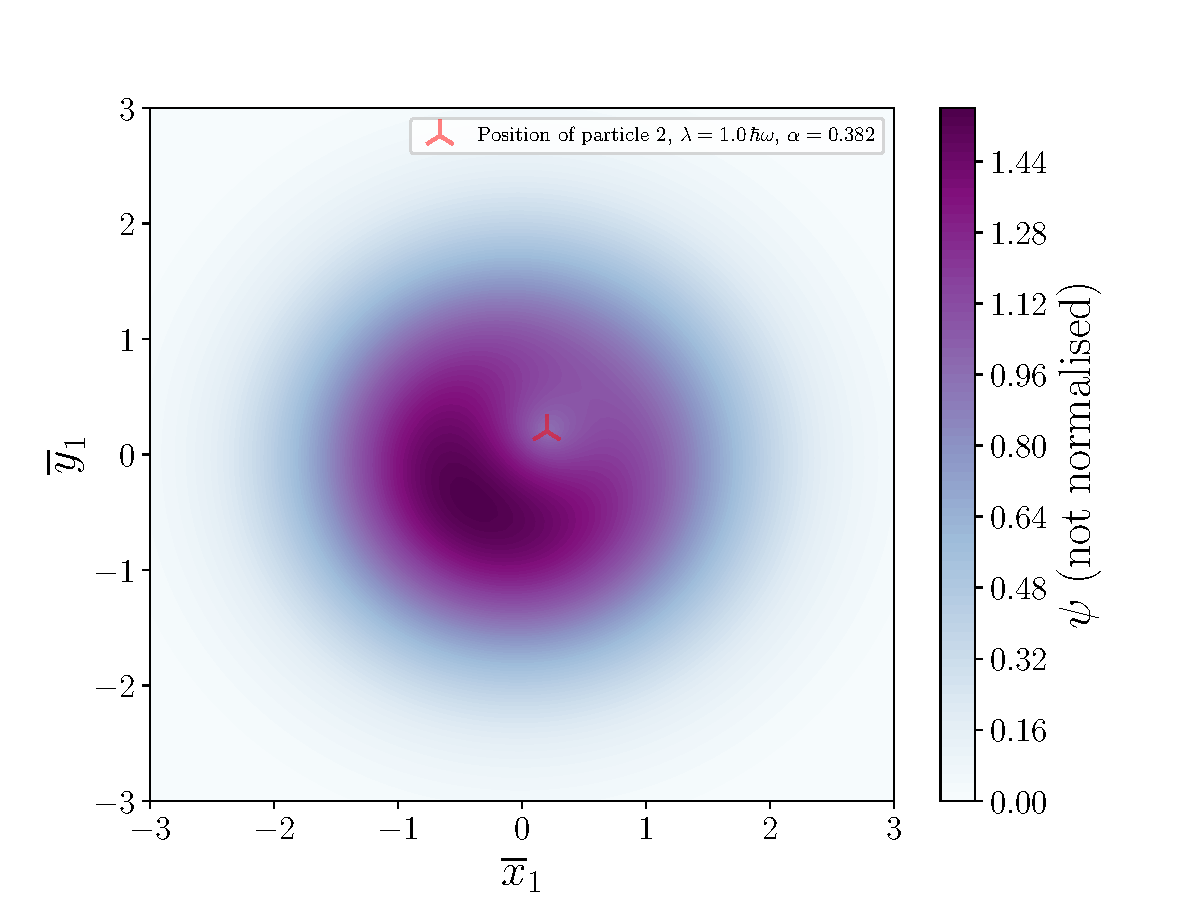
\includegraphics[width=\textwidth]{../plots/wf/wf_02_02_lambda1.pdf}
        \caption{$\lambda=1, \vec{x}_2 = (0.2, 0.2)$}
        \label{subfig:wf_02_02_1}
    \end{subfigure}
    \begin{subfigure}{0.32\textwidth}
        \centering
        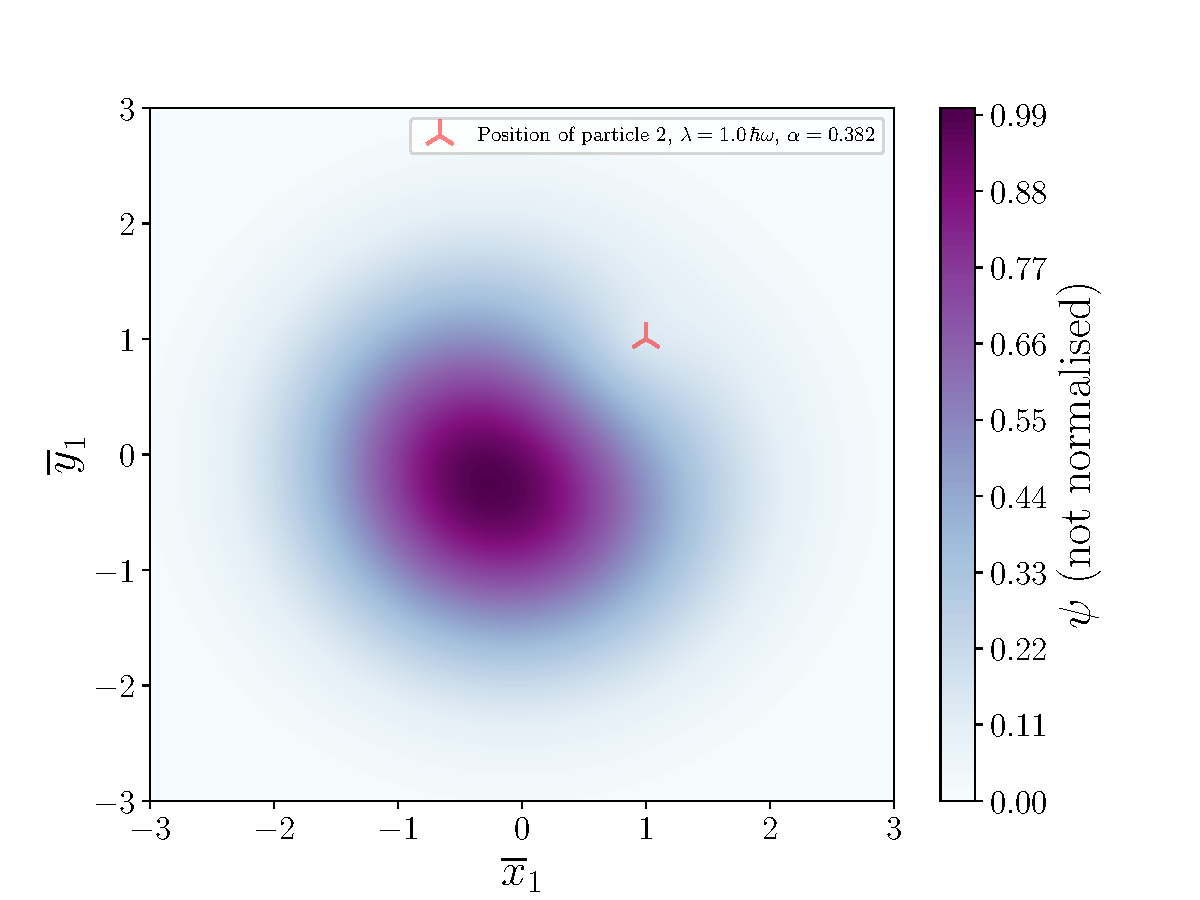
\includegraphics[width=\textwidth]{../plots/wf/wf_1_1_lambda1.pdf}
        \caption{$\lambda=1, \vec{x}_2 = (1, 1)$}
        \label{subfig:wf_1_1_1}
    \end{subfigure} \\
    \begin{subfigure}{0.32\textwidth}
        \centering
        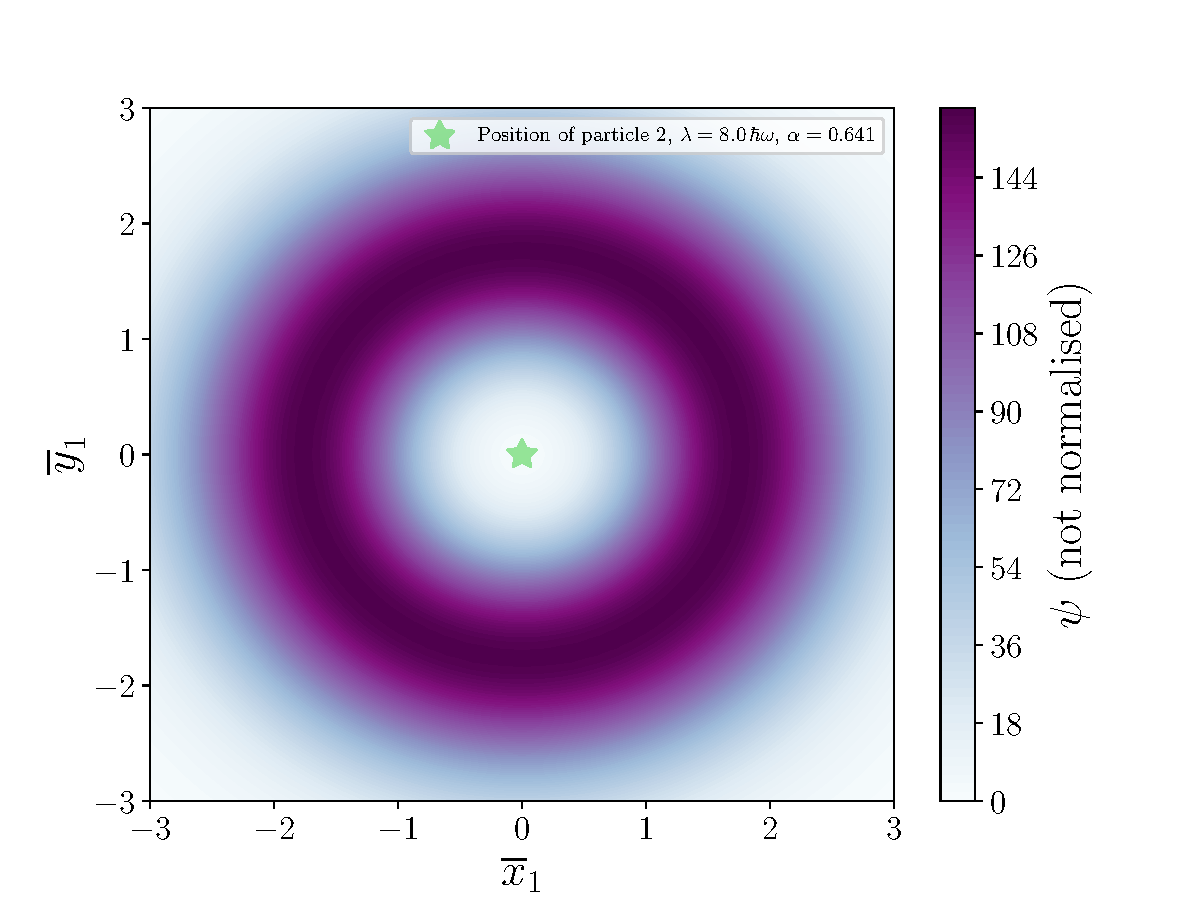
\includegraphics[width=\textwidth]{../plots/wf/wf_0_0_lambda8.pdf}
        \caption{$\lambda=8, \vec{x}_2 = (0, 0)$}
        \label{subfig:wf_0_0_8}
    \end{subfigure}
    \begin{subfigure}{0.32\textwidth}
        \centering
        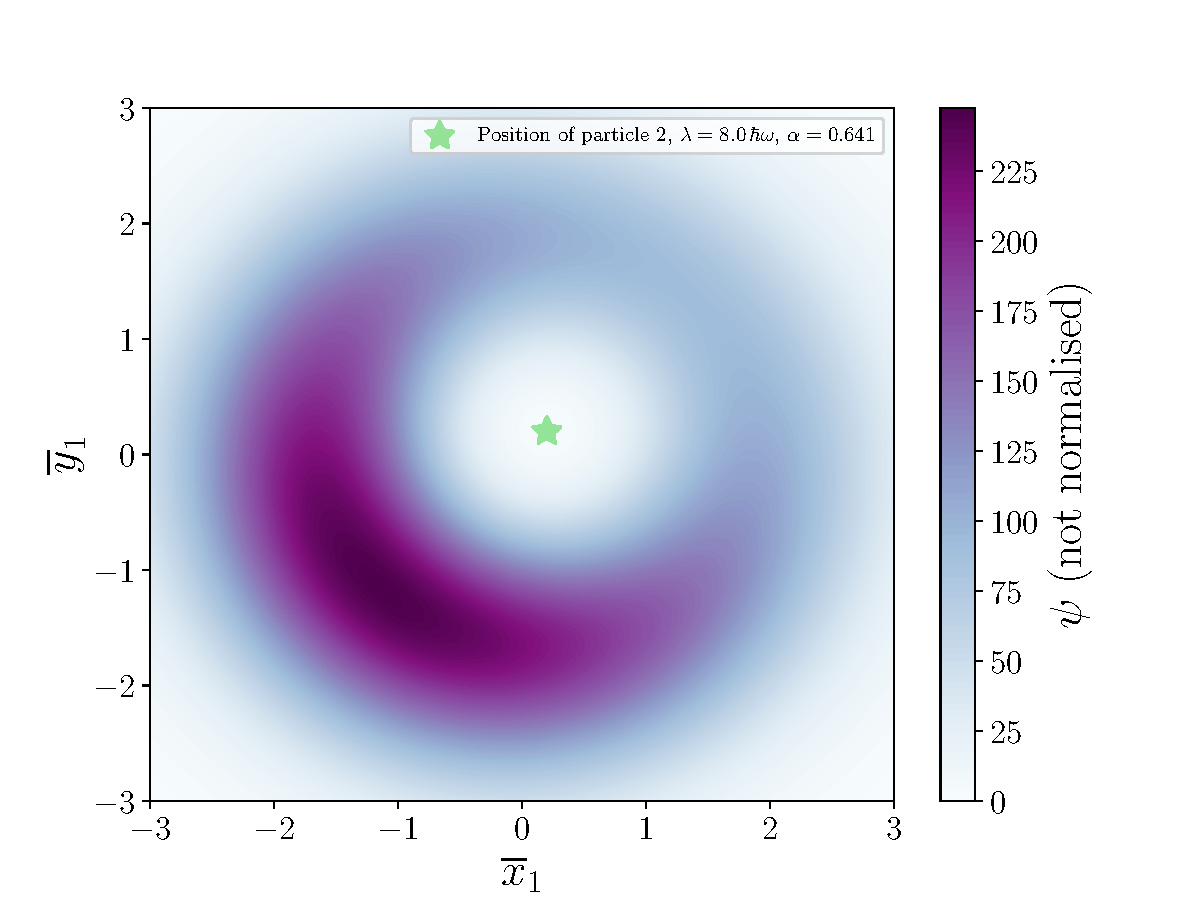
\includegraphics[width=\textwidth]{../plots/wf/wf_02_02_lambda8.pdf}
        \caption{$\lambda=8, \vec{x}_2 = (0.2, 0.2)$}
        \label{subfig:wf_02_02_8}
    \end{subfigure}
    \begin{subfigure}{0.32\textwidth}
        \centering
        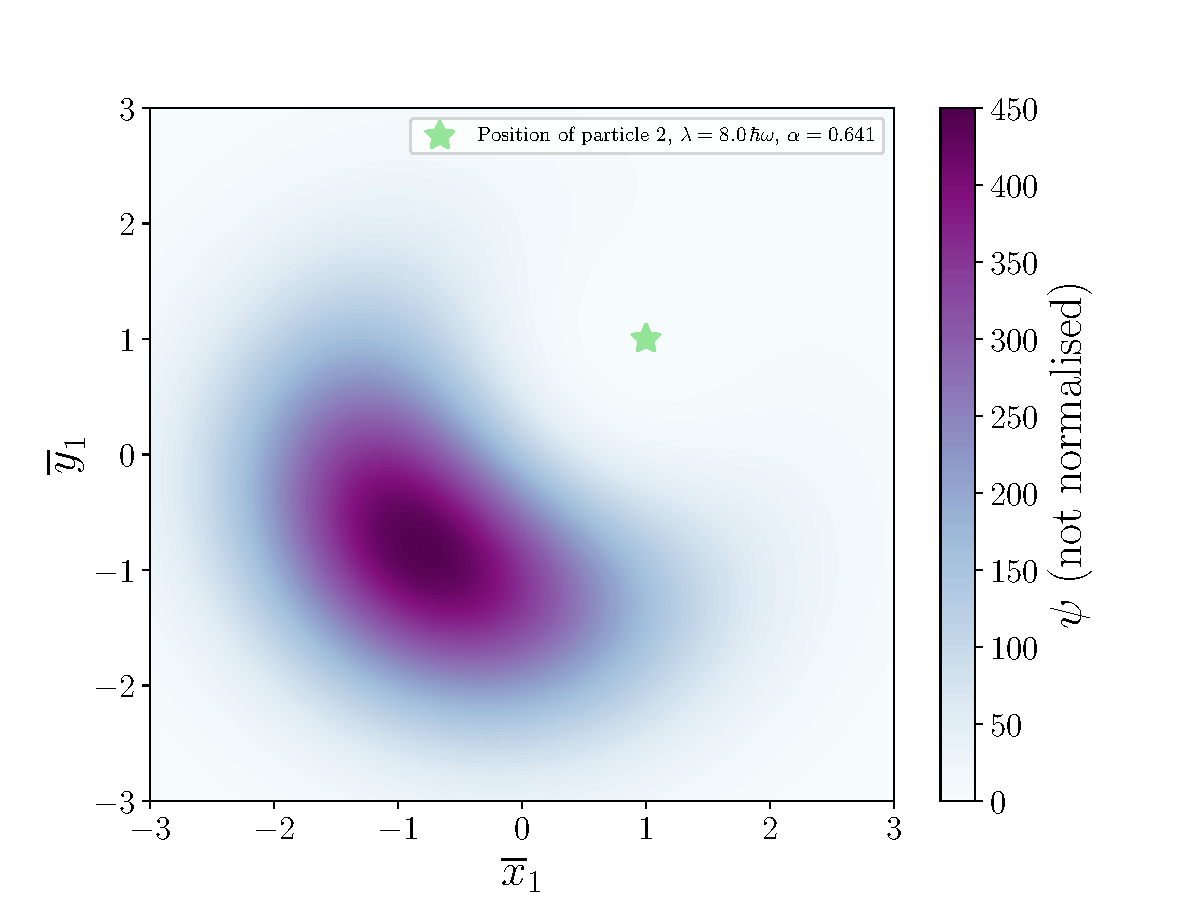
\includegraphics[width=\textwidth]{../plots/wf/wf_1_1_lambda8.pdf}
        \caption{$\lambda=8, \vec{x}_2 = (1, 1)$}
        \label{subfig:wf_1_1_8}
    \end{subfigure} \\
    \caption{Best estimate of the ground state wave function if one of the particles is in a fixed position. Increasing $\lambda$ increases repulsion, as expected.}
    \label{fig:wf}
\end{figure}

Figure~\ref{fig:wf} shows the best estimate of the ground state wave function if one of the particles, e.g.\ particle 2 (the real space part of the wave function is symmetric in exchanging the particles because the trial wave function describes a singlet), is in a fixed position. We observe that the position of particle 2 does not influence the wave function \enquote{of the other particle} since the two particles don't feel each other's presence. This is also why the energy for $\lambda=0$ is exactly that of four one-dimensional harmonic oscillators, i.e. $E=2\hbar\omega$.

For non-zero $\lambda$, we can see that the particles \enquote{avoid each other}, and this happens ever so stronger if $\lambda$ is increased.

\FloatBarrier
\newpage
\section{Conclusion}
In this project, we successfully implemented the described Monte Carlo scheme and tested it for a 1d harmonic oscillator and a 2d, two particle harmonic oscillator with Coulomb repulsion. We were able to reproduce exact results known for special cases.

\newpage
\FloatBarrier
\fakesection{References}
\printbibliography


\end{document}
